\title{Lab 8: Launching Your Payload}
\author{Engineering 100-950}
\date{Winter 2020}
\documentclass[12pt]{article}
\usepackage[margin=1in]{geometry}
\usepackage{fancyhdr}
\chead{Written and Edited by Sarah Redman, Sept. 2019}
\usepackage{hyperref}
\usepackage{circuitikz}
\begin{document}
	\maketitle
	\thispagestyle{fancy}
	
	\section*{Introduction}
	The information in the document should help you understand your launch role and prepare your teams to launch your payload. First and foremost, fill out your availability on the Launch Day Logistics Spreadsheet, and bold your name if you can drive. We understand that not everybody is free for every possible launch day. Ideally, at least two members of your team will be able to go on the launch with your payload. 
	
	\section*{Safety}
	Safety is the most important consideration of the day. The safety manager is the ultimate authority, and it is essential that you pay attention to their instructions. 
	
	Helium tanks are highly pressurized and can turn into missiles if not handled properly. They must be properly strapped into the trailer or transported with dollies. If the helium tank is being transported over rough ground, like grass, it should be rolled.
	
	The driver of every vehicle must be completely focused on driving, not contacting other vehicles or navigating. Their phone number should not be on the contact list, they should not be the contact for their vehicle. The navigator should provide the driver with instructions so that the driver never needs to look at a map or read directions while driving. Do not distract your driver. 
	
	At the launch site, do not leave objects lying around on the ground. The goal is to eliminate trip hazards and be as safe as possible around the helium tanks. After the launch, it is important that the chase car leaves calmly and safely and the clean-up crew thoroughly cleans the area.
	
	\section*{Launch Day Roles}
	Launch roles allow us to efficiently complete everything that needs to happen for a successful launch. Though safety manager, predictions and materials manager are roles will be filled by SPACE 584 students or Professors and IA's, it can be interesting you to take a look at some of these as a team. Predictions Manager is especially hands-on, and often relevant to your science questions. Anybody on the launch can be assigned a car role. It is important to understand what is expected of you and make sure you are ready to fill the role. Ask us any questions you may have.
	
	\subsection*{Safety Manager}
	The safety manager must remain vigilant throughout the launch to ensure all safety considerations are being followed. They are the ultimate authority on safety.
	
	\subsection*{Predictions Manager}
	The Predictions Manager is in charge of checking launch day weather and running predictions of the flight up until the launch using the University of Michigan Balloon Flight Prediction Page. \href{http://vmr.engin.umich.edu/Model/_balloon/index.py}{(Click here to access this tool).} This tool works up to three days ahead of the launch. The purpose of the predictions manager job is twofold:
	\begin{enumerate}
	    \item To identify safe and reasonable launch tracks with desirable launch and landing locations.
	    
	    \item Once we are sure we will be launching that day, to be the resident expert on the predicted track, and watch the track for changes in the hours leading up to the launch.
	\end{enumerate}
	
	To decide if a proposed launch date is reasonable, enter different launch locations and check the length of the launch track, the direction of the balloon track, and that the balloon lands in our favored landing area ("the golden rectangle"). The launch track should be short enough that we do not have to drive more than two hours to get to the launch, and we do not have to drive more than 45 minutes to get back to Ann Arbor. The shorter the better. See Figures 1 and 2 below for direction of the balloon track and our favored landing location. Once a reasonable launch track has been identified, search for possible launch locations near the beginning of the track. Re-run predictions with these locations to find a good track with the best launch location. Schools, public parks, and sports fields are ideal.
	
	\begin{figure}[h!]
		\begin{center}
			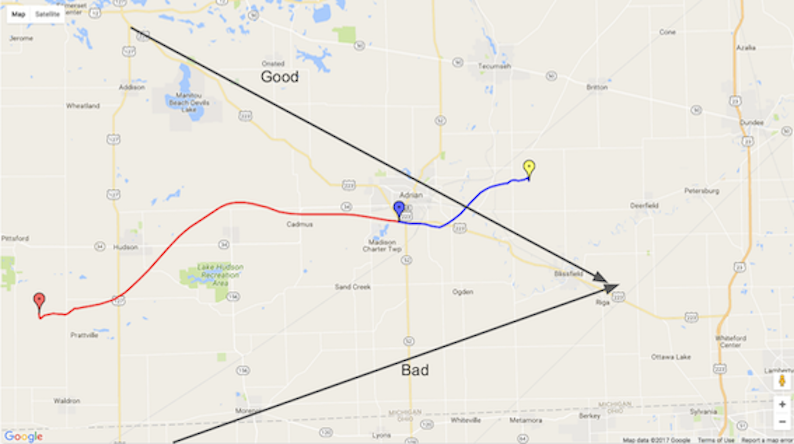
\includegraphics[width = 100mm]{Figures/TrackDirection.png}
			\caption{We prefer to head southeast towards the golden rectangle. (PC: Aaron Ridley, 2017)}
		\end{center}
	\end{figure}
	
	\begin{figure}[h!]
		\begin{center}
			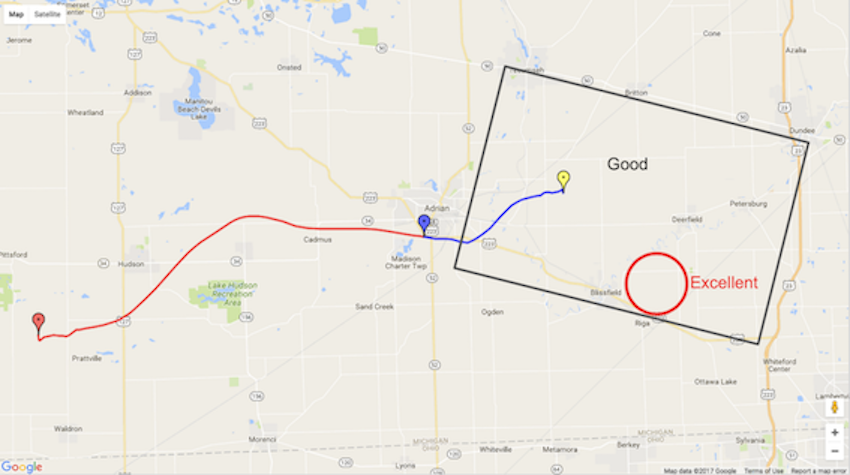
\includegraphics[width = 100mm]{Figures/LandingLocation.png}
			\caption{This is our 'golden rectangle', between Blissfield, Dundee, Tecumseh, and Adrian. (PC: Aaron Ridley, 2017)}
		\end{center}
	\end{figure}
	
	\subsection*{Materials Manager}
	It is the materials manager's job to prepare all materials from the launch day checklist for launch and ensure they get packed into the trailer/a vehicle to come with us. All materials should be ready, labelled, and packed. 
	
	\subsection*{Car Roles}
	\begin{itemize}
	    \item The Driver's sole responsibility is to drive from point A to point B.
	    
	    \item The Navigator needs to be able to read maps and clearly communicate all directions to the driver. They should know where the car and the balloon are at all times.
	    
	    \item Communications will keep the vehicle in contact with other vehicles. Their phone number will be listed as the contact number for the vehicle. They should keep the navigator updated.
	    
	    \item The Tracker is responsible for knowing where the balloon is, how its track is differing from the predictions and updating the navigator on burst and landing.
	\end{itemize}
	
	\section*{Launch Information}
	Once we arrive at the launch site, help lay your payload out in the appropriate payload train. You should know which train and your payload's order in the train from the final go-no go. Make SURE your payload is attached. Shortly before launch/upon direction, turn your payloads on. One member from each team will hold the payload for launch. Be sure somebody is filming and/or taking photos as well! After the launch, the chase car must leave immediately. Make sure you know whether or not you are in the chase car before launch, so they don't have to spend time hunting you down. Remaining vehicles will clean up the launch site before following the chase car.
	
	\section*{Recovery Information}
	This is an exciting part of the day, and also the part of the day where communication is most disjointed. Throughout the recovery, be sure to keep other vehicles updated as to your vehicle's whereabouts.
	Do not go into people's yards and fields without permission. Just because you cannot see a house next to a field does not mean it is public property - it belongs to somebody. Find the nearest house, politely knock on their door and explain the scenario. Send students wearing Michigan gear to do this, it helps with our credibility. Do not enter into any unsafe scenarios to get the payload, e.g. climbing a tree, entering a lake, or walking into a high traffic road.
	
	\section*{Launch Day Schedule}
	\subsection*{The 3 Days Before Launch}
	\begin{itemize}
	    \item Run predictions to determine exact launch day, location,  and track.
	    \item Identify accurate payload train masses.
	    \item Fill out Launch Day Logistics Spreadsheet.
	    \item Assign and prepare for launch roles.
	    \item Prepare payload to balloon connection lines.
	\end{itemize}
	
	\subsection*{The Day Before Launch}
	\begin{itemize}
    	\item Finalize location and launch day logistics.
	    \item Pack all supplies.
	    \item Charge all batteries (IMPORTANT!).
	    \item Pack lunches/snacks, as we may or may not stop for lunch on the way.
	    \item Attend the final Go/No-Go
	\end{itemize}   
	\subsection*{Launch Day}
	This schedule is approximate and launch day sometimes runs longer. Be prepared for this possibility. 
	\begin{itemize}
	    \item 08:00 \quad Arrive at the CSRB
	    \item 09:00 \quad Depart for launch location
	    \item 10:30 \quad Arrive at launch location
	    \item 11:30 \quad Launch
	    \item 13:30 \quad Recovery starts
	    \item 14:30 \quad Head back to CSRB
	    \item 15:30 \quad Arrive at CSRB and unpack gear
	    \item 16:00 \quad Finish with launch day
	\end{itemize}
	
	\section*{Conclusion}
	We hope each of you has a chance to experience a launch with the class. It is a very fun time. Remember to be safe and adhere to any roles you may have been given. If you are unsure about anything, ask any Professor or IA at any time.
\end{document}
